\documentclass[a4paper,11pt,dvipdfmx]{jsarticle}


% 数式
\usepackage{amsmath,amsfonts}
\usepackage{bm}

% 画像
\usepackage[dvipdfmx]{graphicx}

% 図形
\usepackage{tikz}
\usetikzlibrary{shapes.geometric}
\usetikzlibrary {shapes.misc}
\usepackage{tikz-imagelabels}

% ソースコード
\usepackage{listings,jlisting,color}
\lstset{
basicstyle={\ttfamily},
identifierstyle={\small},
commentstyle={\smallitshape},
keywordstyle={\small\bfseries},
ndkeywordstyle={\small},
stringstyle={\small\ttfamily},
frame={tb},
breaklines=true,
columns=[l]{fullflexible},
numbers=left,
xrightmargin=0zw,
xleftmargin=3zw,
numberstyle={\scriptsize},
stepnumber=1,
numbersep=1zw,
lineskip=-0.5ex
}
\renewcommand{\lstlistingname}{ソースコード}


\begin{document}

\title{画像処理 課題1 トーンマッピング}
\author{21T2166D 渡辺大樹}
\date{2023/05/25}
\maketitle

\section{課題の目的・意図}
本課題では、ヒストグラムの幅(画像の輝度値の範囲)を広げる線形濃度変換と
逆光時などの明るさにばらつきが出た画像のヒストグラムの局所的、急激な変化の山を改善するヒストグラム平坦化を
用いて、コントラストの強調された、また明るさのばらつきが少ない画像を得ることを目的とし行う。

\section{処理内容}
以下では線形濃度変換とヒストグラム平坦化の二つの処理で実際に行っていることを説明していく。
\subsection{線形濃度変換}
線形濃度変換では低コントラスト、言い換えれば露出度が適切ではない画像の輝度値を解析し、その分布範囲を線形関数
を用いて広くすることで、色差の大きい画像を生成する。すなわち図\ref{hist_1}のような変換を行う。
\begin{figure}[htbp]
    \centering
    \begin{minipage}{0.4\hsize}
        \centering
        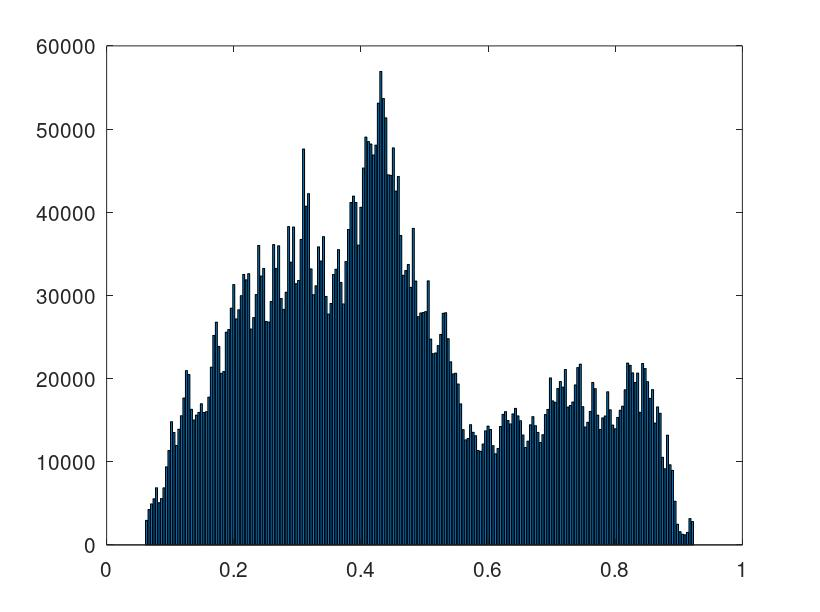
\includegraphics[width=50mm]{./img/linear_ex.jpg}
    \end{minipage}
    \begin{minipage}{0.1\hsize}
        \centering
        \begin{math}
                \overset{f(x)=ax+b}{\to}
        \end{math}
    \end{minipage}
    \begin{minipage}{0.4\hsize}
        \centering
        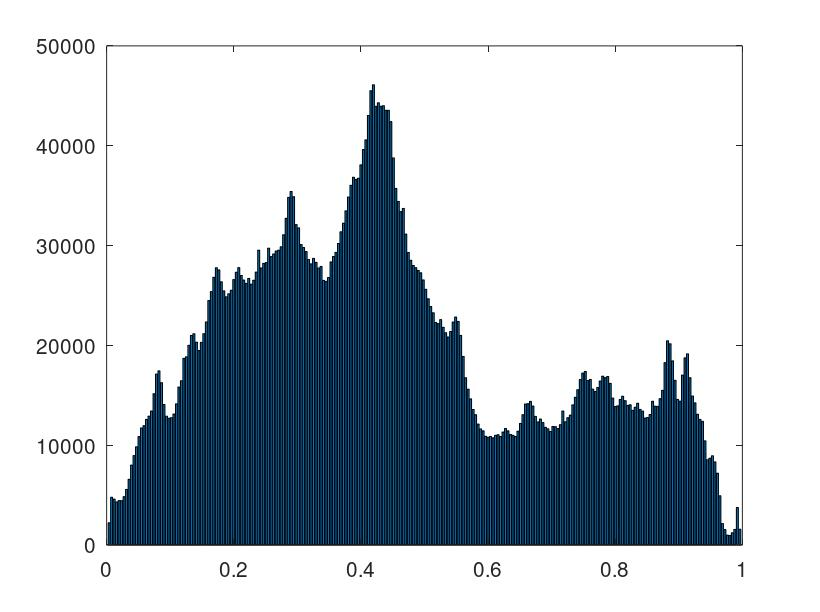
\includegraphics[width=50mm]{./img/linear_ex1.jpg}
    \end{minipage}
    \caption{線形濃度変換によるヒストグラムの変化例}
    \label{hist_1}
\end{figure}

そのためには処理前の画像から得られた輝度値から、その輝度値の範囲を確認。この変換前の輝度値の範囲を$x_1,x_2(x_1<x_2)$とすると、
これを輝度値の最大、最小値まで拡大するような線形関数を、この画像の輝度値全体に適応する必要がある。

入力画像の輝度値の範囲を$x_1,x_2$とし、出力画像の輝度値の範囲を$y_1,y_2$とする。

$y=ax+b$の形の線形関数を用いて変形を行うとき(この変形はアフィン変換という)定数である$a,b$は連立方程式

\begin{equation}
    \left \{ \,
    \begin{aligned}
        y_1 &= ax_1 + b \\
        y_2 &= ax_2 + b
    \end{aligned}
    \right .
\end{equation}
を解くことで求まる。これは$a,b$の係数行列と$(a,b)$の積であると考えれば

\begin{equation}
    \begin{pmatrix}
        y_1 \\ y_2
    \end{pmatrix}
    =
    \begin{pmatrix}
        x_1 & 1 \\
        x_2 & 1
    \end{pmatrix}
    \begin{pmatrix}
        a \\ b
    \end{pmatrix}
\end{equation}
となる。これは逆行列を用いて解くことができて、

\begin{equation}
    \frac{1}{x_1-x_2}
    \begin{pmatrix}
        y_1 - y_2 \\ -x_2y_1 + x_1y_2
    \end{pmatrix}
    =
    \begin{pmatrix}
        a \\ b
    \end{pmatrix}
\end{equation}
としてしまえば、

\begin{equation}
    \left \{ \,
    \begin{aligned}
        a &= \frac{y_1-y_2}{x_1-x_2} \\
        b &= \frac{-x_2y_1+x_1y_2}{x_1-x_2}
    \end{aligned}
    \right .
\end{equation}
と求まる。

\end{document}